\begin{examplebox}
  \textbf{\textcolor{CExample}{例 1｜不用计算，直接判正负（基础）}}

  \textbf{题目：}判断 (1) $\log_2 7$；(2) $\log_2 0.3$；(3) $\log_{0.4}0.6$；(4) $\log_{0.4}1.2$；(5) $\log_3 1$ 的符号。

  \textbf{最快思路：}先确认底数合法、真数为正，然后只比较底数和真数与 $1$ 的大小。
  \[
    \begin{array}{c|c|c|c}
      \text{对数}&\text{底数的位置}&\text{真数的位置}&\text{符号}\\ \hline
      \log_2 7 &>1&>1&+\\
      \log_2 0.3 &>1&<1&-\\
      \log_{0.4}0.6 &<1&<1&+\\
      \log_{0.4}1.2 &<1&>1&-\\
      \log_3 1 &>1&=1&0
    \end{array}
  \]
  \begin{center}
  \begin{tikzpicture}[x=.9cm,y=.8cm,>=stealth]
    \draw[->,thick] (0,0)--(10,0);
    \fill (5,0) circle (2pt) node[below] {$1$};
    \node[above,align=center,teal!75!black] at (2.45,.35) {$0.3,\ 0.4,\ 0.6$\\小于 $1$};
    \node[above,align=center,orange!80!black] at (7.65,.35) {$1.2,\ 2,\ 3,\ 7$\\大于 $1$};
    \draw[very thick,teal!75!black] (1,0)--(4.65,0);
    \draw[very thick,orange!80!black] (5.35,0)--(9.2,0);
  \end{tikzpicture}

  \end{center}
  \textbf{答案：}$+,-,+,-,0$。\textbf{提醒：}不要把“真数小于 $1$”直接理解为“对数为负”；还要看底数。

  \medskip
  \textbf{\textcolor{CExample}{例 2｜真数含参数，怎样一眼判号？（提高）}}

  \textbf{题目：}已知 $a>0$ 且 $a\neq1$，判断 $\log_a(a^2+1)$ 的符号。

  \textbf{第一步：只看真数。}因为 $a>0$，有 $a^2>0$，所以 $a^2+1>1$，真数一定在 $1$ 的右侧。

  \textbf{第二步：只看底数。}如果 $a>1$，底和真都大于 $1$，对数为正；如果 $0<a<1$，底小于 $1$ 而真大于 $1$，对数为负。
  \[
    \boxed{\log_a(a^2+1)\begin{cases}>0,&a>1,\\<0,&0<a<1.\end{cases}}
  \]
  \begin{center}
  \begin{tikzpicture}[x=.9cm,y=.8cm,>=stealth]
    \draw[->,thick] (0,0)--(9.5,0) node[right] {$a$};
    \draw[very thick,orange!80!black] (.7,0)--(4.2,0);
    \draw[very thick,teal!75!black] (4.2,0)--(8.8,0);
    \draw (4.2,0) circle (2.5pt) node[below] {$1$};
    \node[orange!80!black,above] at (2.3,.25) {$0<a<1: \text{负}$};
    \node[teal!75!black,above] at (6.6,.25) {$a>1: \text{正}$};
    \node[below,gray] at (4.2,-.9) {$a=1$ 不允许};
  \end{tikzpicture}

  \end{center}
  \textbf{为什么这题快？}不用算 $a^2+1$ 的具体值，只需抓住它\textbf{始终大于 $1$}。

  \medskip
  \textbf{\textcolor{CExample}{例 3｜带参数的对数不等式（综合）}}

  \textbf{题目：}已知 $a>0,\ a\neq1$，解 $\log_a(x^2-3x+2)>0$。

  \textbf{第一步：先守住定义域。}令 $u=x^2-3x+2=(x-1)(x-2)$，真数必须大于 $0$：
  \[u>0\iff x<1\ \text{或}\ x>2.\]
  \textbf{第二步：对数大于零，意味着什么？}
  \begin{itemize}[leftmargin=*,itemsep=0.25em,topsep=0.25em]
    \item 若 $a>1$，必须 $u>1$，即 $x^2-3x+1>0$。
    \item 若 $0<a<1$，必须 $0<u<1$，即同时满足 $x^2-3x+2>0$ 和 $x^2-3x+1<0$。
  \end{itemize}
  \textbf{第三步：解二次不等式。}设
  \[r_1=\frac{3-\sqrt5}{2},\qquad r_2=\frac{3+\sqrt5}{2}.
  \]
  因为 $x^2-3x+1=(x-r_1)(x-r_2)$，所以它在 $r_1,r_2$ 之外为正，在二者之间为负。注意 $r_1<1<2<r_2$。
  \begin{center}
  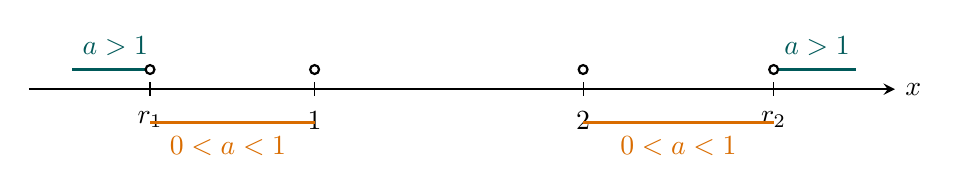
\begin{tikzpicture}[x=1.1cm,y=1cm,>=stealth]
    \draw[->,thick] (0,0)--(10,0) node[right] {$x$};
    \foreach \x/\lab in {1.4/$r_1$,3.3/$1$,6.4/$2$,8.6/$r_2$} {
      \draw (\x,.09)--(\x,-.09) node[below=2pt] {\lab};
    }
    \draw[very thick,teal!70!black] (.5,.25)--(1.4,.25);
    \draw[very thick,teal!70!black] (8.6,.25)--(9.55,.25);
    \node[above,teal!70!black] at (1.0,.3) {$a>1$};
    \node[above,teal!70!black] at (9.1,.3) {$a>1$};
    \draw[very thick,orange!85!black] (1.4,-.42)--(3.3,-.42);
    \draw[very thick,orange!85!black] (6.4,-.42)--(8.6,-.42);
    \node[below,orange!85!black] at (2.3,-.48) {$0<a<1$};
    \node[below,orange!85!black] at (7.5,-.48) {$0<a<1$};
    \foreach \x in {1.4,3.3,6.4,8.6} {\draw[fill=white,thick] (\x,.25) circle (1.6pt);}
  \end{tikzpicture}

  \end{center}
  \textbf{答案：}
  \[
  \boxed{\begin{aligned}
    a>1:\quad &x\in(-\infty,r_1)\cup(r_2,+\infty),\\[2pt]
    0<a<1:\quad &x\in(r_1,1)\cup(2,r_2).
  \end{aligned}}
  \]
  \textbf{最容易漏的步骤：}当 $0<a<1$ 时，光有 $u<1$ 还不够，\textbf{必须同时有 $u>0$}；上面数轴中 $[1,2]$ 一段正是被定义域排除的。

  \medskip
  \textbf{\textcolor{CExample}{考场速用三步：}}\textbf{先验真数 $>0$，再和 $1$ 比大小，最后解普通不等式。}
\end{examplebox}
